\section{Exercises on Network Flow Problems}

\subsection{Problem 3.1. Transportation Schedules}

\paragraph{}
\begin{quote}
GTC manufactures its network cables at six different factories in the country. From these factories, the cables are transported to the 44 cable depots, which are warehouses in different parts of the country. From the cable depots the cables are transported to the places were they are actually demanded.
Figure \ref{network3-1} contains a schematic road map of 50 locations, labeled 1, ..., 50. Factories where the network cables are manufactured are located in the locations 8, 11, 21, 24, 33, and 36. After production, the cable is stored on spools. The total production of each factory is given in units of ten cable spools. This number is given next to the factory location in Figure \ref{network3-1}. The remaining 44 locations in Figure \ref{network3-1} refer to the 44 cable depots, where the cable spools are stored until they are needed. The demand of the various depots is the number next to the corresponding node in Figure \ref{network3-1} (also in units of ten spools, and with a negative sign). The spools are transported by means of trucks which always carry precisely ten spools; the transportation costs per truck, called ``truck costs'', are shown as numbers next to the corresponding road segments in the network of Figure \ref{network3-1}.
\end{quote}

\begin{figure}[H]
	\centering
	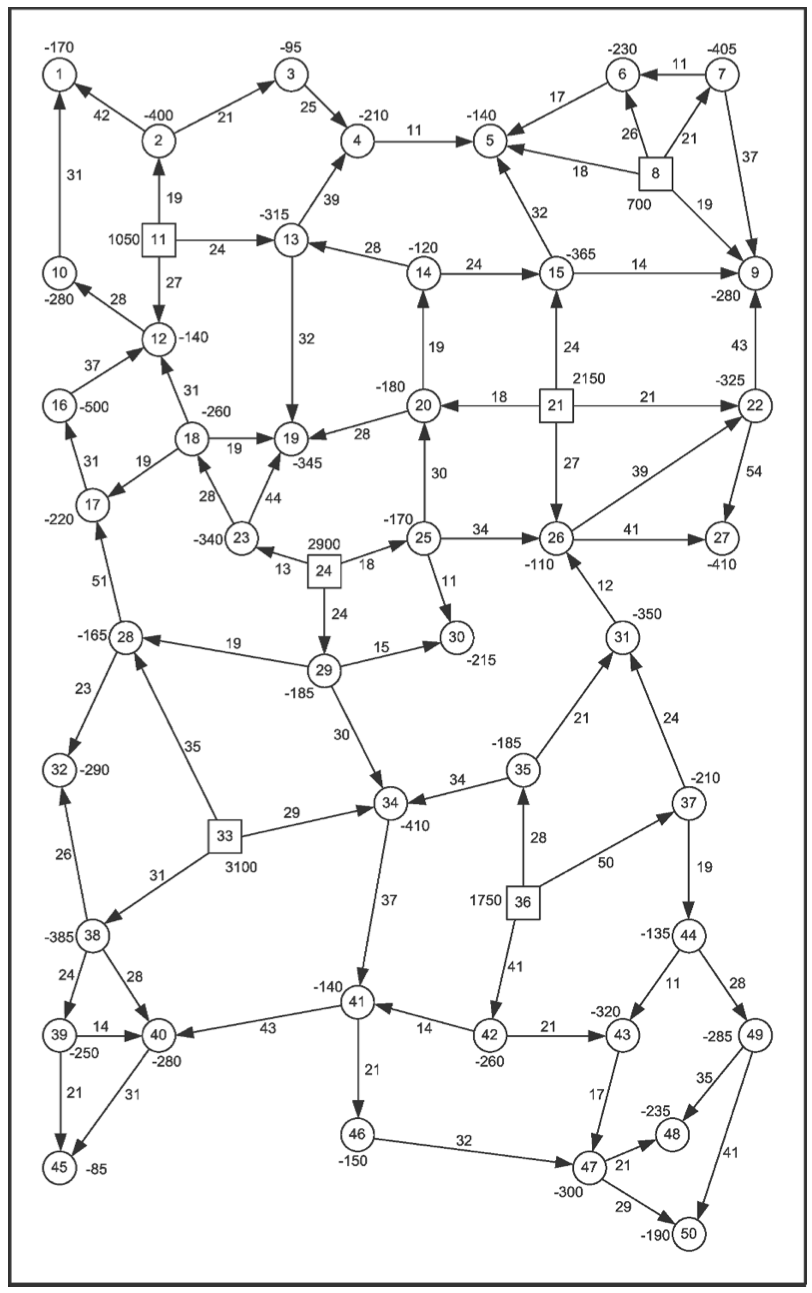
\includegraphics[scale=1]{./img/figure3-13.png}
	\caption{Supplies, demands (in units of 10 spools), and truck costs (in \texteuro) on a road map with 50 locations}
	\label{network3-1}
\end{figure}

\paragraph{(a)}
\begin{quote}
GTC wants to know a cheapest way of transporting spools to the cable depots in such a way that all depot demands are satisfied.
Since more spools are produced than are demanded, the company also wants to know which factories manufacture spools that are not shipped. How many spools are left at these factories?
\end{quote}

\paragraph{}
We find the minimum cost maximum flow in a network obtained from figure \ref{network3-1}. The capacities of arcs are infinite, the costs are taken from figure \ref{network3-1}. To 50 existing vertices we added a source and a sink. We added arcs from source to the 6 depots with zero costs and capacities equal to the number of spools in depots. We added arcs from all demand locations to sink with zero costs and capacities equal to the number of demanded spools. The number of spools left at factories can be found as the capacities of edges from source in residual network. We found minimum cost maximum flow and checked that it has saturated all arcs to the sink (i.e. all demand is satisfied).

\paragraph{}
Each arc (except the arcs incident to sink or source) in our graph corresponds to a road. The flow through an arc in our graph corresponds to the number of spools transported through it. The arcs from source spread incoming flow among depots and limit the flow from each depot. The arcs to sink aggregate the flow from demand locations and limit the demand of each location. The flow through edges can be used as a transportation plan right away. It can be more convenient to have a transportation plan as a list of routes from source depots to demand locations, so that a truck can be assigned to each route. We found both representations. We obtained the second representation from the first one using greedy algorithm.

\paragraph{}
For finding the minimum cost maximum flow we use Ford-Fulkerson-like algorithm that on each step finds the cheapest augmenting path using Ford-Bellman algorithm. We could have used Dijkstra's algorithm with potentials, but it would be an overkill for such small graph.

\paragraph{}
The flow as a list of flows through edges is shown in figure \ref{flow3-1a}. The transportation plan as a list of routes is shown in table \ref{flow3-1a-paths}. The minimum total cost is \texteuro 578,535. The number of remaining spools is shown in table \ref{spools-left}.

\begin{figure}[H]
\centering
\begin{multicols}{5}
$ 2 \rightarrow 1 $ : 170

$ 2 \rightarrow 3 $ : 95

$ 8 \rightarrow 5 $ : 65

$ 8 \rightarrow 6 $ : 230

$ 8 \rightarrow 7 $ : 405
$ 11 \rightarrow 2 $ : 665
$ 11 \rightarrow 13 $ : 385
$ 12 \rightarrow 10 $ : 280
$ 13 \rightarrow 4 $ : 210
$ 14 \rightarrow 13 $ : 140
$ 15 \rightarrow 5 $ : 75
$ 15 \rightarrow 9 $ : 280
$ 17 \rightarrow 16 $ : 500
$ 18 \rightarrow 12 $ : 420
$ 18 \rightarrow 17 $ : 720
$ 20 \rightarrow 14 $ : 260
$ 20 \rightarrow 19 $ : 145
$ 21 \rightarrow 15 $ : 720
$ 21 \rightarrow 20 $ : 585
$ 21 \rightarrow 22 $ : 325
$ 21 \rightarrow 26 $ : 520
$ 23 \rightarrow 18 $ : 1400
$ 23 \rightarrow 19 $ : 200
$ 24 \rightarrow 23 $ : 1940
$ 24 \rightarrow 25 $ : 385
$ 24 \rightarrow 29 $ : 185
$ 25 \rightarrow 30 $ : 215
$ 26 \rightarrow 27 $ : 410
$ 33 \rightarrow 28 $ : 165
$ 33 \rightarrow 34 $ : 1420
$ 33 \rightarrow 38 $ : 1290
$ 34 \rightarrow 41 $ : 1010
$ 35 \rightarrow 31 $ : 350
$ 36 \rightarrow 35 $ : 535
$ 36 \rightarrow 37 $ : 630
$ 36 \rightarrow 42 $ : 585
$ 37 \rightarrow 44 $ : 420
$ 38 \rightarrow 32 $ : 290
$ 38 \rightarrow 39 $ : 335
$ 38 \rightarrow 40 $ : 280
$ 39 \rightarrow 45 $ : 85
$ 41 \rightarrow 46 $ : 870
$ 42 \rightarrow 43 $ : 325
$ 43 \rightarrow 47 $ : 5
$ 44 \rightarrow 49 $ : 285
$ 46 \rightarrow 47 $ : 720
$ 47 \rightarrow 48 $ : 235
$ 47 \rightarrow 50 $ : 190
\end{multicols}
\caption{Optimal transportation plan: the flow through each arc in tens of spools}
\label{flow3-1a}
\end{figure}

\begin{table}[H]
\centering
\begin{tabular}{|r|l|l|}
\hline
Path & Tens of spools & Cost \\ \hline
$ 8 \rightarrow 5 $ & 65 & \texteuro 1170\\ \hline
$ 8 \rightarrow 6 $ & 230 & \texteuro 5980\\ \hline
$ 8 \rightarrow 7 $ & 405 & \texteuro 8505\\ \hline
$ 11 \rightarrow 2 $ & 400 & \texteuro 7600\\ \hline
$ 11 \rightarrow 2 \rightarrow 1 $ & 170 & \texteuro 10370\\ \hline
$ 11 \rightarrow 2 \rightarrow 3 $ & 95 & \texteuro 3800\\ \hline
$ 11 \rightarrow 13 $ & 315 & \texteuro 7560\\ \hline
$ 11 \rightarrow 13 \rightarrow 4 $ & 70 & \texteuro 4410\\ \hline
$ 21 \rightarrow 15 $ & 365 & \texteuro 8760\\ \hline
$ 21 \rightarrow 15 \rightarrow 5 $ & 75 & \texteuro 4200\\ \hline
$ 21 \rightarrow 15 \rightarrow 9 $ & 280 & \texteuro 10640\\ \hline
$ 21 \rightarrow 20 $ & 180 & \texteuro 3240\\ \hline
$ 21 \rightarrow 20 \rightarrow 14 $ & 120 & \texteuro 4440\\ \hline
$ 21 \rightarrow 20 \rightarrow 14 \rightarrow 13 \rightarrow 4 $ & 140 & \texteuro 14560\\ \hline
$ 21 \rightarrow 20 \rightarrow 19 $ & 145 & \texteuro 6670\\ \hline
$ 21 \rightarrow 22 $ & 325 & \texteuro 6825\\ \hline
$ 21 \rightarrow 26 $ & 110 & \texteuro 2970\\ \hline
$ 21 \rightarrow 26 \rightarrow 27 $ & 410 & \texteuro 27880\\ \hline
$ 24 \rightarrow 23 $ & 340 & \texteuro 4420\\ \hline
$ 24 \rightarrow 23 \rightarrow 18 $ & 260 & \texteuro 10660\\ \hline
$ 24 \rightarrow 23 \rightarrow 18 \rightarrow 12 $ & 140 & \texteuro 10080\\ \hline
$ 24 \rightarrow 23 \rightarrow 18 \rightarrow 12 \rightarrow 10 $ & 280 & \texteuro 28000\\ \hline
$ 24 \rightarrow 23 \rightarrow 18 \rightarrow 17 $ & 220 & \texteuro 13200\\ \hline
$ 24 \rightarrow 23 \rightarrow 18 \rightarrow 17 \rightarrow 16 $ & 500 & \texteuro 45500\\ \hline
$ 24 \rightarrow 23 \rightarrow 19 $ & 200 & \texteuro 11400\\ \hline
$ 24 \rightarrow 25 $ & 170 & \texteuro 3060\\ \hline
$ 24 \rightarrow 25 \rightarrow 30 $ & 215 & \texteuro 6235\\ \hline
$ 24 \rightarrow 29 $ & 185 & \texteuro 4440\\ \hline
$ 33 \rightarrow 28 $ & 165 & \texteuro 5775\\ \hline
$ 33 \rightarrow 34 $ & 410 & \texteuro 11890\\ \hline
$ 33 \rightarrow 34 \rightarrow 41 $ & 140 & \texteuro 9240\\ \hline
$ 33 \rightarrow 34 \rightarrow 41 \rightarrow 46 $ & 150 & \texteuro 13050\\ \hline
$ 33 \rightarrow 34 \rightarrow 41 \rightarrow 46 \rightarrow 47 $ & 300 & \texteuro 35700\\ \hline
$ 33 \rightarrow 34 \rightarrow 41 \rightarrow 46 \rightarrow 47 \rightarrow 48 $ & 235 & \texteuro 32900\\ \hline
$ 33 \rightarrow 34 \rightarrow 41 \rightarrow 46 \rightarrow 47 \rightarrow 50 $ & 185 & \texteuro 27380\\ \hline
$ 33 \rightarrow 38 $ & 385 & \texteuro 11935\\ \hline
$ 33 \rightarrow 38 \rightarrow 32 $ & 290 & \texteuro 16530\\ \hline
$ 33 \rightarrow 38 \rightarrow 39 $ & 250 & \texteuro 13750\\ \hline
$ 33 \rightarrow 38 \rightarrow 39 \rightarrow 45 $ & 85 & \texteuro 6460\\ \hline
$ 33 \rightarrow 38 \rightarrow 40 $ & 280 & \texteuro 16520\\ \hline
$ 36 \rightarrow 35 $ & 185 & \texteuro 5180\\ \hline
$ 36 \rightarrow 35 \rightarrow 31 $ & 350 & \texteuro 17150\\ \hline
$ 36 \rightarrow 37 $ & 210 & \texteuro 10500\\ \hline
$ 36 \rightarrow 37 \rightarrow 44 $ & 135 & \texteuro 9315\\ \hline
$ 36 \rightarrow 37 \rightarrow 44 \rightarrow 49 $ & 285 & \texteuro 27645\\ \hline
$ 36 \rightarrow 42 $ & 260 & \texteuro 10660\\ \hline
$ 36 \rightarrow 42 \rightarrow 43 $ & 320 & \texteuro 19840\\ \hline
$ 36 \rightarrow 42 \rightarrow 43 \rightarrow 47 \rightarrow 50 $ & 5 & \texteuro 540\\ \hline
\end{tabular}
\caption{Optimal transportation plan decomposed into paths}
\label{flow3-1a-paths}
\end{table}

\begin{table}[H]
\centering
\begin{tabular}{|r|c|c|c|c|c|c|}
\hline
factory & 8 & 11 & 21 & 24 & 33 & 36 \\ \hline
spools & 0 & 0 & 0 & 390 & 225 & 0   \\ \hline
\end{tabular}
\caption{Number of spools left on each factory}
\label{spools-left}
\end{table}

\paragraph{(b)}
\begin{quote}
There are rumors that, because of the heavy traffic, the government is considering to levy toll on vehicles that use a certain road segment. It is not known yet which segment would be taxed, but road segments 38 $\rightarrow$ 40, 33 $\rightarrow$ 38, 12 $\rightarrow$ 10, 35 $\rightarrow$ 31, and 29 $\rightarrow$ 34 are considered as the most likely ones.
GTC is wondering whether the change of one road segment into a toll road will affect the cheapest transportation schedule from Problem 3.3(a). Determine for each of the above five road segments the maximum toll fee that can be charged on that segment without the current transportation plan becoming costlier than some other plan.
\end{quote}

\paragraph{}
We need to find the upper tolerance of some edges (by definition of upper tolerance). To find the upper tolerance of an edge we set its capacity to the flow through it minus one and find the minimum cost maximum flow again. The difference between costs is the upper tolerance.

\paragraph{}
The maximum toll fees are given in table \ref{toll-fees}.

\begin{table}[H]
\centering
\begin{tabular}{|c|c|l|}
\hline
Arc & Fee & Comment \\ \hline
$ 38 \rightarrow 40 $ & 10 & \\ \hline
$ 33 \rightarrow 38 $ & 1 & \\ \hline
$ 12 \rightarrow 10 $ & $+\infty$ & can't reach 10 without this arc \\ \hline
$ 35 \rightarrow 31 $ & 25 & \\ \hline
$ 29 \rightarrow 34 $ & $+\infty$ & not in optimal plan \\ \hline
\end{tabular}
\caption{Maximum toll fees not changing the plan}
\label{toll-fees}
\end{table}

\paragraph{(c)}
\begin{quote}
There is also a possibility that the direction of traffic on the road segment 33~$\rightarrow$~34 will be reversed, i.e., it will become a one-way-traffic from 34 to 33. Determine a cheapest transportation plan under this new circumstance.
\end{quote}

\paragraph{}
We reversed the arc and found the flow again. The new flow is shown in figure \ref{flow3-1c}. The new transportation plan as a list of routes is shown in table \ref{flow3-1c-paths}. Its cost is \texteuro 658,175.

\begin{figure}[H]
\centering
\begin{multicols}{5}
$ 2 \rightarrow 1 $ : 170

$ 2 \rightarrow 3 $ : 95

$ 8 \rightarrow 5 $ : 65

$ 8 \rightarrow 6 $ : 230

$ 8 \rightarrow 7 $ : 405
$ 11 \rightarrow 2 $ : 665
$ 11 \rightarrow 13 $ : 385
$ 12 \rightarrow 10 $ : 280
$ 13 \rightarrow 4 $ : 210
$ 14 \rightarrow 13 $ : 140
$ 15 \rightarrow 5 $ : 75
$ 15 \rightarrow 9 $ : 280
$ 16 \rightarrow 12 $ : 310
$ 17 \rightarrow 16 $ : 810
$ 18 \rightarrow 12 $ : 110
$ 20 \rightarrow 14 $ : 260
$ 20 \rightarrow 19 $ : 145
$ 21 \rightarrow 15 $ : 720
$ 21 \rightarrow 20 $ : 585
$ 21 \rightarrow 22 $ : 325
$ 21 \rightarrow 26 $ : 520
$ 23 \rightarrow 18 $ : 370
$ 23 \rightarrow 19 $ : 200
$ 24 \rightarrow 23 $ : 910
$ 24 \rightarrow 25 $ : 385
$ 24 \rightarrow 29 $ : 1605
$ 25 \rightarrow 30 $ : 215
$ 26 \rightarrow 27 $ : 410
$ 28 \rightarrow 17 $ : 1030
$ 29 \rightarrow 34 $ : 1420
$ 33 \rightarrow 28 $ : 1195
$ 33 \rightarrow 38 $ : 1290
$ 34 \rightarrow 41 $ : 1010
$ 35 \rightarrow 31 $ : 350
$ 36 \rightarrow 35 $ : 535
$ 36 \rightarrow 37 $ : 630
$ 36 \rightarrow 42 $ : 585
$ 37 \rightarrow 44 $ : 420
$ 38 \rightarrow 32 $ : 290
$ 38 \rightarrow 39 $ : 335
$ 38 \rightarrow 40 $ : 280
$ 39 \rightarrow 45 $ : 85
$ 41 \rightarrow 46 $ : 870
$ 42 \rightarrow 43 $ : 325
$ 43 \rightarrow 47 $ : 5
$ 44 \rightarrow 49 $ : 285
$ 46 \rightarrow 47 $ : 720
$ 47 \rightarrow 48 $ : 235
$ 47 \rightarrow 50 $ : 190
\end{multicols}
\caption{Optimal transportation plan with reversed arc}
\label{flow3-1c}
\end{figure}

\begin{table}[H]
\centering
\begin{tabular}{|r|l|l|}
\hline
Path & Tens of spools & Cost \\ \hline
$ 8 \rightarrow 5 $ & 65 & \texteuro 1170\\ \hline
$ 8 \rightarrow 6 $ & 230 & \texteuro 5980\\ \hline
$ 8 \rightarrow 7 $ & 405 & \texteuro 8505\\ \hline
$ 11 \rightarrow 2 $ & 400 & \texteuro 7600\\ \hline
$ 11 \rightarrow 2 \rightarrow 1 $ & 170 & \texteuro 10370\\ \hline
$ 11 \rightarrow 2 \rightarrow 3 $ & 95 & \texteuro 3800\\ \hline
$ 11 \rightarrow 13 $ & 315 & \texteuro 7560\\ \hline
$ 11 \rightarrow 13 \rightarrow 4 $ & 70 & \texteuro 4410\\ \hline
$ 21 \rightarrow 15 $ & 365 & \texteuro 8760\\ \hline
$ 21 \rightarrow 15 \rightarrow 5 $ & 75 & \texteuro 4200\\ \hline
$ 21 \rightarrow 15 \rightarrow 9 $ & 280 & \texteuro 10640\\ \hline
$ 21 \rightarrow 20 $ & 180 & \texteuro 3240\\ \hline
$ 21 \rightarrow 20 \rightarrow 14 $ & 120 & \texteuro 4440\\ \hline
$ 21 \rightarrow 20 \rightarrow 14 \rightarrow 13 \rightarrow 4 $ & 140 & \texteuro 14560\\ \hline
$ 21 \rightarrow 20 \rightarrow 19 $ & 145 & \texteuro 6670\\ \hline
$ 21 \rightarrow 22 $ & 325 & \texteuro 6825\\ \hline
$ 21 \rightarrow 26 $ & 110 & \texteuro 2970\\ \hline
$ 21 \rightarrow 26 \rightarrow 27 $ & 410 & \texteuro 27880\\ \hline
$ 24 \rightarrow 23 $ & 340 & \texteuro 4420\\ \hline
$ 24 \rightarrow 23 \rightarrow 18 $ & 260 & \texteuro 10660\\ \hline
$ 24 \rightarrow 23 \rightarrow 18 \rightarrow 12 $ & 110 & \texteuro 7920\\ \hline
$ 24 \rightarrow 23 \rightarrow 19 $ & 200 & \texteuro 11400\\ \hline
$ 24 \rightarrow 25 $ & 170 & \texteuro 3060\\ \hline
$ 24 \rightarrow 25 \rightarrow 30 $ & 215 & \texteuro 6235\\ \hline
$ 24 \rightarrow 29 $ & 185 & \texteuro 4440\\ \hline
$ 24 \rightarrow 29 \rightarrow 34 $ & 410 & \texteuro 22140\\ \hline
$ 24 \rightarrow 29 \rightarrow 34 \rightarrow 41 $ & 140 & \texteuro 12740\\ \hline
$ 24 \rightarrow 29 \rightarrow 34 \rightarrow 41 \rightarrow 46 $ & 150 & \texteuro 16800\\ \hline
$ 24 \rightarrow 29 \rightarrow 34 \rightarrow 41 \rightarrow 46 \rightarrow 47 $ & 300 & \texteuro 43200\\ \hline
$ 24 \rightarrow 29 \rightarrow 34 \rightarrow 41 \rightarrow 46 \rightarrow 47 \rightarrow 48 $ & 235 & \texteuro 38775\\ \hline
$ 24 \rightarrow 29 \rightarrow 34 \rightarrow 41 \rightarrow 46 \rightarrow 47 \rightarrow 50 $ & 185 & \texteuro 32005\\ \hline
$ 33 \rightarrow 28 $ & 165 & \texteuro 5775\\ \hline
$ 33 \rightarrow 28 \rightarrow 17 $ & 220 & \texteuro 18920\\ \hline
$ 33 \rightarrow 28 \rightarrow 17 \rightarrow 16 $ & 500 & \texteuro 58500\\ \hline
$ 33 \rightarrow 28 \rightarrow 17 \rightarrow 16 \rightarrow 12 $ & 30 & \texteuro 4620\\ \hline
$ 33 \rightarrow 28 \rightarrow 17 \rightarrow 16 \rightarrow 12 \rightarrow 10 $ & 280 & \texteuro 50960\\ \hline
$ 33 \rightarrow 38 $ & 385 & \texteuro 11935\\ \hline
$ 33 \rightarrow 38 \rightarrow 32 $ & 290 & \texteuro 16530\\ \hline
$ 33 \rightarrow 38 \rightarrow 39 $ & 250 & \texteuro 13750\\ \hline
$ 33 \rightarrow 38 \rightarrow 39 \rightarrow 45 $ & 85 & \texteuro 6460\\ \hline
$ 33 \rightarrow 38 \rightarrow 40 $ & 280 & \texteuro 16520\\ \hline
$ 36 \rightarrow 35 $ & 185 & \texteuro 5180\\ \hline
$ 36 \rightarrow 35 \rightarrow 31 $ & 350 & \texteuro 17150\\ \hline
$ 36 \rightarrow 37 $ & 210 & \texteuro 10500\\ \hline
$ 36 \rightarrow 37 \rightarrow 44 $ & 135 & \texteuro 9315\\ \hline
$ 36 \rightarrow 37 \rightarrow 44 \rightarrow 49 $ & 285 & \texteuro 27645\\ \hline
$ 36 \rightarrow 42 $ & 260 & \texteuro 10660\\ \hline
$ 36 \rightarrow 42 \rightarrow 43 $ & 320 & \texteuro 19840\\ \hline
$ 36 \rightarrow 42 \rightarrow 43 \rightarrow 47 \rightarrow 50 $ & 5 & \texteuro 540\\ \hline
\end{tabular}
\caption{Optimal transportation plan decomposed into paths}
\label{flow3-1c-paths}
\end{table}
